\documentclass[authoryear, review, 11pt]{elsarticle}

\setlength{\textwidth}{6.5in}
%\setlength{\textheight}{9in}
\setlength{\topmargin}{0in}
\setlength{\oddsidemargin}{0in}
\setlength{\evensidemargin}{0in}

\usepackage{amsmath}
\usepackage{amsthm}
\usepackage{amssymb}
\usepackage{mathabx}
\usepackage{bm}
\usepackage{multirow}

%\geometry{landscape}                % Activate for for rotated page geometry
\usepackage[parfill]{parskip}    % Activate to begin paragraphs with an empty line rather than an indent
\usepackage{graphicx}
\usepackage{epstopdf}
\usepackage{natbib}
\usepackage{verbatim}
\usepackage{longtable}
\usepackage{rotating}
\usepackage[nolists,nomarkers]{endfloat}
\DeclareDelayedFloatFlavour{sidewaystable}{table}

\usepackage{relsize}
%\usepackage{caption}
\usepackage{subcaption}
\usepackage{fullpage}
\usepackage{booktabs}


\usepackage{setspace}
\setstretch{2}

\DeclareGraphicsRule{.tif}{png}{.png}{`convert #1 `dirname #1`/`basename #1 .tif`.png}
\DeclareMathOperator*{\argmin}{\arg\!\min}
\DeclareMathOperator*{\argmax}{\arg\!\max}
\DeclareMathOperator*{\bw}{\mbox{bw}}
\DeclareMathOperator*{\df}{\mbox{df}}
\newcommand{\vect}[1]{\bm{#1}}
\newcommand{\E}{\mathop{\mathbb E}}


\title{Local Variable Selection and Parameter Estimation of Spatially Varying Coefficient Regression Models}
\author{Wesley Brooks}
\date{}                                           % Activate to display a given date or no date

\begin{document}
\maketitle
%\section{}
%\subsection{}

%Pastebin:
%Spatial association - meaning that nearby locations are more alike than distant locations - is a key concept in spatial statistics.\
%for univariate output $y$, $p$-vector of covariates $\bm{x}$, and random noise $\varepsilon$ all indexed by location $\bm{s}
%where $\phi$ is a bandwidth parameter and $\delta(\bm{s}, \bm{t})$ is the Euclidean distance between locations $\bm{s}$ and $\bm{t}$.

%\begin{spacing}{2}
\section{Introduction}
	%Varying coefficient regression
	Whereas the coefficients in traditional linear regression are scalar constants, the coefficients in a varying coefficient regression (VCR) model are functions - often \emph{smooth} functions - of some effect modifying variable \citep{Hastie:1993a}. When the effect modifying variable represents location in a spatial domain, a VCR model implies a spatially local regression model such that the regression coefficients vary over space and will be referred to as a spatially varying coefficient regression model (SVCR). Statistical inference for the coefficients as functions of location in an SVCR model is more complicated than estimating the coefficients in a global linear regression model where the coefficients are constant across the spatial domain. This document concerns the development of new methodologies for the analysis of spatial data using SVCR.
	
	%Spatial data / spatial regression
	The methodology described herein is applicable to geostatistical data and areal data. Let $\mathcal{D}$ be a spatial domain on which data is collected. For geostatistical data, let $\bm{s}$ denote a location in $\mathcal{D}$. Let univariate $\left\{Y(\bm{s}) : \bm{s} \in \mathcal{D}\right\}$ and possibly multivariate $\left\{\bm{X}(\bm{s}) : \bm{s} \in \mathcal{D}\right\}$ denote random fields of the response and the covariates, respectively. For $i = 1, \dots, n$, let $\bm{s}_i$ denote the location in $\mathcal{D}$ of the $i$th observation of the response and the covariates. Then the data are a realization of the random variables $\left\{Y(\bm{s}_i), \bm{X}(\bm{s}_i)\right\}$ for $i=1, \dots, n$. Let the observed data be denoted $\left\{y(\bm{s}_i), \bm{x}(\bm{s}_i)\right\}$, $i=1, \dots, n$.
	
	For areal data, the spatial domain $\mathcal{D}$ is partitioned into $n$ regions $\{D_1, \dots, D_n\}$ such that $\mathcal{D} = \bigcup \limits_{i=1}^nD_i$. In the case of areal data, the random variables $\left\{Y(D_i), \bm{X}(D_i)\right\}$ are defined for regions instead of for point locations; population and spatial mean temperature are examples of areal data. The analytical method described herein can be applied to areal data if they are recast as geostatistical data by assuming that the data are point-referenced to a representative location of each region, such as the centroid. That is, $\left\{\bm{X}(\bm{s}_i), Y(\bm{s}_i)\right\} $ where $\bm{s}_i$ is the centroid of $D_i$ for $i=i, \dots, n$.
	
	 Common practice in the analysis of geostatistical and areal data is to model the response variable with a spatial linear regression model consisting of the sum of a fixed mean function, a spatial random effect, and random error all on domain $\mathcal{D}$, as in: 
\begin{align}\label{eq:spatial-regression}
    Y(\bm{s}) = \bm{X}(\bm{s})'\bm{\beta} + W(\bm{s}) + \varepsilon(\bm{s})
\end{align}
where $\bm{X}(\bm{s})'\bm{\beta}$ is the mean function consisting of a vector of covariates $\bm{X}(\bm{s})$, and a vector of regression coefficients $\bm{\beta}$. The random error $\varepsilon(\bm{s})$ denotes white noise such that the errors are independent and identically distributed with mean zero and variance $\sigma^2$, while the random component $W(\bm{s})$ denotes a mean-zero, second-order stationary random field that is independent of the random error. The mean function captures the large-scale systematic trend of the response, the spatial random field $W(\bm{s})$ can be thought of as a small-scale spatial random effect, and the error term $\varepsilon(\bm{s})$ captures micro-scale variation \citep{Cressie:1993}. It is common to pre-specify the form of a covariance function for the spatial random effect $W(\bm{s})$ \citep{Diggle:2007}. For example, the exponential covariance function (a special case of the Mat\'{e}rn class of covariance functions) has the form
\begin{align}\label{eq:exponential-covariance}
    \text{Cov}(W(\bm{s}), W(\bm{t})) = \exp\left\{-\phi^{-1} \delta(\bm{s}, \bm{t}) \right\}
\end{align}
where $\phi$ denotes a range parameter and $\delta(\bm{s}, \bm{t})$ denotes the Euclidean distance between locations $\bm{s}$ and $\bm{t}$. The general form of a covariance function in the Mat\'{e}rn class is
\begin{align}\label{eq:matern-covarinace}
    \text{Cov}(W(\bm{s}), W(\bm{t})) = \left\{\Gamma(\nu) 2^{\nu-1} \right\}^{-1} \left\{\delta(\bm{s}, \bm{t}) \phi^{-1}\sqrt{2\nu}\right\}^\nu K_{\nu} \left(\delta(\bm{s}, \bm{t}) \phi^{-1}\sqrt{2\nu}\right)
    \end{align}
where $\nu$ denotes the degree of smoothness, $K_{\nu}$ denotes the modified Bessel equation of the second kind, and as before $\phi$ denotes a range parameter and $\delta(\bm{s}, \bm{t})$ the Euclidean distance between locations $\bm{s}$ and $\bm{t}$. The exponential covariance function corresponds to a Mat\'{e}rn class covariance function with $\nu = 1/2$.

	%SVCR - justification
	%Stationarity in spatial linear regression
	A random field is said to be stationary if the joint distribution of a the response at a finite set of locations does not change when the set of locations are all shifted in space by a fixed spatial lag. That is, letting $\left\{T(\bm{s}) : \bm{s} \in \mathcal{D}\right\}$ be a random field on spatial domain $\mathcal{D}$ that takes value $T(\bm{s}_i)$ at location $\bm{s}_i \in \mathcal{D}$ for $i = 1, \dots, n$, the random field $T(\bm{s})$ is stationary if $F_n\left(T(\bm{s}_1), \dots, T(\bm{s}_n)\right) = F_n\left(T(\bm{s}_1+\bm{h}), \dots, T(\bm{s}_n+\bm{h})\right)$ where $F_n(\cdot)$ is the joint distribution of a length $n$ sample from $T(\bm{s})$ and $\bm{h}$ is a fixed spatial lag. A random field is second-order stationary if the joint distribution at any two locations in the domain does not change when the locations are shifted by a fixed spatial lag.
	
	The coefficient vector $\bm{\beta}$ in (\ref{eq:spatial-regression}) is a fixed constant. The model can be made more flexible if the coefficients are described by a stationary random field. Such a model is written
\begin{align}\label{eq:SVCR-process}
    Y(\bm{s}) = \bm{X}(\bm{s})'\bm{\beta}(\bm{s}) + \varepsilon(\bm{s})
\end{align}
	where $\bm{\beta}(\bm{s})$ is a random coefficient field with a Mat\'{e}rn-class covariance function and the spatial random effect $W(\bm{s})$ included in the intercept $\beta_0(\bm{s})$. The random coefficient field $\bm{\beta}(\bm{s})$ can be estimated by Markov Chain Monte Carlo (MCMC) methods under the assumption that $\bm{\beta}(\bm{s})$ is stationary \citep{Gelfand:2003}.

	%The spatial random effect describes the spatial pattern in the deviations from the systematic part of the model. When fitting the spatial regression model (\ref{eq:spatial-regression}), it is usually required that the the fitted values of the spatial random effect and of the residuals sum to zero, i.e. $\sum\limits_{i=1}^n\hat{W}(\bm{s}_i) = 0$ and $\sum\limits_{i=1}^n\hat{\varepsilon}(\bm{s}_i) = 0$. This mode of analysis is appropriate when the systematic part of the regression model does not vary between locations. On the other hand, a VCR model is appropriate for the case where the systematic part of the regression model does vary across locations.

	%Spatial VCR
	Alternatively, kernel-based and spline-based methods can be considered for fitting varying coefficient models without assuming the coefficients are described by a stationary random field. For example, it is straightforward to modify a thin plate regression spline model into a traditional, non-spatial VCR model \citep{Wood:2006}. A local likelihood can also be used to fit generalized linear models with varying coefficients using kernel smoothing \citep{Loader:1999}. \cite{Fan:1999} demonstrated that the optimal kernel bandwidth estimate for a VCR model can be found via a two-step technique.
	
	Model selection in VCR models may be local or global. Global selection means including or excluding variables everywhere in the spatial domain, while local selection means including or excluding variables at individual locations within the spatial domain. Two methods have been proposed for global model selection in spline-based VCR models. \cite{Wang:2008a} applied a SCAD penalty \citep{Fan:2001} for variable selection in spline-based VCR models with a univariate effect-modifying variable. \cite{Antoniadis:2012a} used the nonnegative Garrote penalty \citep{Breiman:1995} in P-spline-based VCR models having a univariate effect-modifying variable.
	
	Wavelet methods for fitting SVCR models were explored by \cite{Shang-2011} and \cite{Zhang-2011}. Sparsity in the wavelet coefficients is achieved either by $\ell_1$-penalization (also known as the Lasso \citep{Tibshirani:1996}) \citep{Shang-2011} or by Bayesian variable selection \citep{Zhang-2011}. Sparsity in the wavelet domain does not imply sparsity in the covariates, though, so neither method can be used for local variable selection.

	%GWR
	Geographically weighted regression (GWR) is a kernel-based method of estimating the coefficients of an SVCR model where the kernel weights are based on the distance between sampling locations \cite{Brundson:1998a, Fotheringham:2002}. At each sampling location, traditional GWR estimates the local regression coefficients by the local likelihood \citep{Loader:1999}. As a kernel-based smoother for regression coefficients, traditional GWR tends to exhibit bias near the boundary of the region being modeled \citep{Hastie:1993b}. One way to reduce the boundary-effect bias is to model the coefficient surface as locally linear rather than locally constant by including coefficient-by-location interactions \cite{Wang:2008b}.
	
	%Local variable selection
	Traditional GWR relies on \emph{a priori} global model selection to decide which variables should be included in the model. In the context of ordinary least squares regression, Lasso regularization for variable selection \citep{Tibshirani:1996}, while popular, does not generally produce consistent estimates of the relevant predictor variables \citep{Leng-2006}. Regularization methods such as the adaptive Lasso (AL) \citep{Zou:2006} were developed and shown to have appealing properties for automating variable selection, sometimes including the ``oracle" property of asymptotically selecting exactly the correct set of covariates for inclusion in a regression model.
	
	The idea of using Lasso regularization for local variable selection in a GWR model appeared in the literature as the geographically weighted Lasso (GWL) \citep{Wheeler:2009}. The GWL uses the Lasso with a jackknife criterion for selection of the tuning parameters. Because the jackknife criterion can only be computed at sampling locations where the response variable is observed, the GWL cannot be used for imputation of missing data nor for interpolation between sampling locations. By using the Lasso for variable selection, the GWL also imports known shortcomings of the Lasso, such as inconsistent model selection \citep{Zou:2006, Leng-2006} and poor prediction accuracy when the covariates are correlated \citep{Tibshirani:1996, Zou:2005}. 
	
	This paper introduces a new regularization method, called the geographically weighted adaptive elastic net (GWAEN), for local variable selection in GWR models that overcomes these limitations of the GWL. A penalized-likelihood criterion to select the GWAEN tuning parameter, which means that a GWAEN can be fit at any location within the domain, whether or not data were observed at that location. In particular, a type of BIC is developed and used herein, but in principle another information criterion like the AIC is also possible. The local BIC presented here is based on the local likelihood \citep{Loader:1999} and a total BIC is based on an \emph{ad hoc} calculation of the sample size and degrees of freedom for estimating the spatially-varying coefficient surfaces.
	
	Model selection under the GWAEN uses the adaptive elastic net (AEN). The AEN achieves an oracle property and performs better than other oracle-like methods when there is collinearity in the covariates \citep{Zou:2009}. The AEN is a combination of a quadratic and a Lasso penalty to the log-likelihood. When the quadratic penalty is zero, the AEN is identical to the adaptive Lasso (AL), and in this case the GWAEN becomes the geographically weighted adaptive Lasso (GWAL). The AL was implemented in two ways - once via the least angle regression (LARS) algorithm \citep{Efron:2004b} which uses least squares, and once via the coordinate descent algorithm using the {\tt R} package {\tt glmnet} \citep{Friedman:2010}. The third regularization method implemented here uses an adaptive elastic net (AEN) penalty \citep{Zou:2009}, also via the coordinate descent algorithm using the {\tt glmnet} package.
	
	The remainder of this document is organized as follows: the traditional GWR is presented in Section \ref{section:GWR}. The geographically weighted adaptive Lasso (GWAL) and geographically weighted adaptive elastic net (GWAEN) are introduced in section \ref{section:model-selection}. Section \ref{section:simulation} Section \ref{section:data-analysis}

\section{Geographically Weighted Regression \label{section:GWR}}
	\subsection{Model}	
	Consider $n$ data observations, taken at sampling locations $\bm{s}_1, \dots, \bm{s}_n$ in a spatial domain $D \subset \mathbb{R}^2$. For $i = 1, \dots, n$, let $y(\bm{s}_i)$ and $\bm{x}(\bm{s}_i)$ denote the univariate response variable, and a $(p+1)$-variate vector of covariates measured at location $\bm{s}_i$, respectively. At each location $\bm{s}_i$, assume that the outcome is related to the covariates by a linear model where the coefficients $\bm{\beta}(\bm{s}_i)$ may be spatially-varying and $\varepsilon(\bm{s}_i)$ is random error at location $\bm{s}_i$. That is,
	\begin{align}\label{eq:lm(s)}
		y(\bm{s}_i) = \bm{x}(\bm{s}_i)' \bm{\beta}(\bm{s}_i) + \varepsilon(\bm{s}_i).
	\end{align}
	
	Further assume that the error term $\varepsilon(\bm{s}_i)$ is normally distributed with zero mean and variance $\sigma^2$, and that $\varepsilon(\bm{s}_i)$, $i=1, \dots, n$ are independent. That is,
	\begin{align} \label{eq:err}
		\varepsilon(\bm{s}_i) \overset{iid}{\sim} \mathcal{N} \left( 0,\sigma^2 \right).
	\end{align}
	
	In order to simplify the notation, let $\bm{x}(\bm{s}_i) \equiv \bm{x}_i \equiv \left( 1, x_{i1}, \dots, x_{ip} \right)'$, $\bm{\beta}(\bm{s}_i) \equiv \bm{\beta}_i \equiv \left(\beta_{i0}, \beta_{i1}, \dots, \beta_{ip} \right)'$, and $y(\bm{s}_i) \equiv y_i$.  Equations (\ref{eq:lm(s)}) and (\ref{eq:err}) can now be rewritten as
	\begin{align}
		y_i = \bm{x}'_i \bm{\beta}_i + \varepsilon_i \text{ and } \varepsilon_i \overset{iid}{\sim} \mathcal{N} \left( 0,\sigma^2 \right).
	\end{align}
	
	Further, let $\bm{X} = \left( \bm{x}_1, \dots, \bm{x}_n \right)'$ and $\bm{y} = \left( y_1, \dots, y_n \right)'$. Thus, conditional on the design matrix $\bm{X}$, observations of the response variable at different locations are independent of each other. Then, a total log-likelihood of the observed data is the sum of the log-likelihood of each individual observation:
	 \begin{align}
	 	\ell\left( \bm{\beta} \right) = - \left(1/2\right) \left\{ n \log \left( 2 \pi \sigma^2\right) +  \left(\sigma^{2}\right)^{-1}  \sum_{i=1}^n \left(y_i - \bm{x}'_i\bm{\beta}_i \right)^2  \right\}.
	\end{align}
	
	Since there are a total of $n \times (p+1)$ free parameters for $n$ observations, the model is not identifiable and it is not possible to directly maximize the total likelihood. One way to effectively reduce the number of parameters is to assume that the coefficients $\bm{\beta}(\bm{s})$ are smoothly varying over space, and use a kernel smoother to make pointwise estimates of the coefficients by maximizing a local likelihood. In the setting of spatial data and with the kernel smoother based on the physical distance between sampling locations, this is the traditional GWR.
		
	\subsection{Estimation}		
	In the traditional GWR, the coefficient surface $\bm{\beta}(\bm{s})$ is estimated at each sampling location $\bm{s}_i$. First calculate the Euclidean distance $\delta_{ii'} \equiv \delta\left(\bm{s}_i, \bm{s}_{i'}\right) \equiv \|\bm{s}_i  -\bm{s}_{i'}\|_2$ between locations $\bm{s}_i$ and $\bm{s}_{i'}$ for all $i, i' = 1, \dots, n$. The bi-square kernel can be used to generate spatial weights based on the Euclidean distances and a bandwidth $\phi$:
	
	\begin{align}\label{eq:bisquare}
		w_{ii'} = \begin{cases} \left[1-\left(\phi^{-1}\delta_{ii'}\right)^2\right]^2 &\mbox{ if } \delta_{ii'} < \phi, \\ 0 &\mbox{ if } \delta_{ii'} \geq \phi. \end{cases}
	\end{align}
	
	The bisquare kernel in (\ref{eq:bisquare}) assigns the maximum weight of one where $\bm{s}_i = \bm{s}_{i'}$ (i.e. $\delta_{ii'}=0$), is continuously differentiable, and assigns zero weight to observations at distances greater than one bandwidth from $\bm{s}_i$. For the purpose of estimation, define a local likelihood at each location:
	\begin{align}\label{eq:local-likelihood}
		\mathcal{L}_i \left(\bm{\beta}_i \right) &= \prod_{i'=1}^n \left[ \left(2 \pi \sigma^2_i  \right)^{-1/2}  \exp\left\{-\left(2 \sigma^2_i\right)^{-1}  \left(y_{i'} - \bm{x}'_{i'} \bm{\beta}_i \right)^2 \right\} \right] ^ {w_{ii'}},
	\end{align}			
	where $\sigma_i^2$ is a local approximation to the error variance $\sigma^2$ \citep{Fotheringham:2002}. Thus, the local log-likelihood function is, up to an additive constant:
	\begin{align}\label{eq:local-log-likelihood}
		\ell_i\left(\bm{\beta}_i\right) &= -(1/2) \sum_{i'=1}^n w_{ii'} \left\{ \log{\sigma^2_i}  + \left(\sigma^2_i\right)^{-1}  \left(y_{i'} - \bm{x}'_{i'} \bm{\beta}_i \right)^2 \right\}.
	\end{align}
	From (\ref{eq:local-likelihood}) and (\ref{eq:local-log-likelihood}), it is apparent that the GWR coefficient estimates $\hat{\bm{\beta}}_{i,\text{GWR}}$ maximizing the local likelihood at location $\bm{s}_i$ can be obtained using weighted least squares. 
	
	 Setting to zero the derivative of (\ref{eq:local-log-likelihood}) with respect to $\sigma_i^2$, the maximum likelihood estimate (MLE) $\hat{\sigma}_i^2$ is found to be:	 
	 \begin{align}
	 	\hat{\sigma}_i^2 = \left(\sum \limits_{i'=1}^{n} w_{ii'} \right)^{-1} \sum \limits_{i'=1}^n w_{ii'}\left(y_{i'} - \bm{x}_{i'}'\hat{\bm{\beta}}_i\right)^2
	\end{align}
	
	\begin{comment}
	\paragraph{Algorithmic details} Both $\hat{\bm{\beta}_i}$ and $\hat{\sigma}_i^2$ can be obtained by the method of least squares. Let $\bm{W}_i$ denote a diagonal weight matrix with diagonal entries $w_{ii'}$ for $i'=1, \dots, n$. That is,
	\begin{align}
		\bm{W}_i =  {\rm diag}\left\{w_{ii'}\right\}_{i' = 1}^n.
	\end{align}
	
	It follows that, by weighted least squares,
	\begin{align}
		\hat{\bm{\beta}}_{i, \text{GWR}} = \left( \bm{X}'\bm{W}_i\bm{X} \right)^{-1} \bm{X}'\bm{W}_i\bm{y}.
	\end{align}
	
	and
	\begin{align}
		\hat{\sigma}^2_i &= \left(\bm{1}_n'\bm{w}_i \right)^{-1} \left(\bm{y}-\bm{X}\left(\bm{X}'\bm{W}_i\bm{X}\right)^{-1}\bm{X}'\bm{W}_i\bm{y}\right)' \bm{W}_i \left(\bm{y}-\bm{X}\left(\bm{X}'\bm{W}_i\bm{X}\right)^{-1}\bm{X}'\bm{W}_i\bm{y}\right) \notag \\
		&= \left(\bm{1}_n'\bm{w}_i \right)^{-1}  \left(\bm{y}-\hat{\bm{y}}\right)' \bm{W}_i \left(\bm{y}-\hat{\bm{y}}\right),
	\end{align}	
	where $\bm{1}_n$ is an $n$-variate vector of ones.
	\end{comment}
	
	\begin{comment}
	Estimation of $\hat{\bm{\beta}}_i$ and $\hat{\sigma}_i$ is by maximum local likelihood, which is implemented by setting the derivatives of (\ref{eq:local-log-likelihood}) to zero:
	\begin{eqnarray}
		\left\{\frac{\partial \ell_i}{\partial \bm{\beta}_i} \right\}_j =   \sum_{i'=1}^n \left\{ x_{i'j} w_{ii'} \sigma^{-2}_i \left( y_{i'} - \bm{x}'_{i'} \bm{\beta}_i \right) \right\} \\
		\frac{\partial \ell_i}{\partial \sigma_i^2} \bigg|_{\hat{\beta}_i} &=& -\frac{1}{2} \sum_{i'=1}^n w_{ii'} \left\{ \left(\sigma_i^{2}\right)^{-1} - \left(\sigma_i^{2}\right)^{-2} \left( y_i - \bm{x}_i'\bm{\hat{\beta}}_i \right)^2 \right\} \\
		\hat{\sigma}_i^2 &=& \left(\sum_{i'=1}^n w_{ii'}\right)^{-1} \sum_{i'=1}^n w_{ii'} \left(y_i - \bm{x}_i'\hat{\bm{\beta}}_i\right)
	\end{eqnarray}
		
		\left\{\frac{\partial^2 \ell_i}{\partial \bm{\beta}_i \partial \bm{\beta}'_i} \right\}_{j,k} = -\sum_{i'=1}^n \left\{ x_{i'j} x_{i'k} w_{ii'} \sigma^{-2}_i \right\}
	\end{eqnarray}
	
	So the observed Fisher information in the locally weighted sample is
	\begin{align}
		\bm{\mathcal{J}}_i &=& \sigma^{-2}_i \left( \begin{array}{ccc} \sum_{i'=1}^n  w_{ii'} x^2_{i'1}   & \dots & \sum_{i'=1}^n w_{ii'} x_{i'1} x_{i'p}   \\ \vdots & \ddots & \vdots \\ \sum_{i'=1}^n  w_{ii'} x_{i'p} x_{i'1}    & \dots & \sum_{i'=1}^n  w_{ii'} x^2_{i'p}  \end{array} \right) \notag\\
		&=& \sigma^{-2}_i \sum_{i'=1}^n w_{ii'}\left( \begin{array}{ccc}  x^2_{i'1} & \dots & x_{i'1} x_{i'p} \\ \vdots & \ddots & \vdots \\ x_{i'p} x_{i'1} & \dots &  x^2_{i'p} \end{array} \right)\notag \\
		&=& \sigma^{-2}_i \sum_{i'=1}^n w_{ii'} \bm{x}_{i'} \bm{x}'_{i'}
	\end{align}	
	
	The form of the observed Fisher information suggests that the information in the data $\bm{x}_{i'}$ about the coefficients at location $s_i$ is proportional to the weight $w_{ii'}$.
	\end{comment}

	
	 
	
\section{Model Selection \label{section:model-selection}}
	\subsection{Local Variable Selection}
	Both the AL and the AEN are explored as penalty functions for local variable selection in GWR models.
	
	The proposed local variable selection with AL penalty is an $\ell_1$ regularization method for variable selection in regression models \citep{Zou:2006}. Unlike the traditional Lasso penalty, which applies an equal penalty to each covariate in the local model at $\bm{s}_i$, the AL adjusts the penalty of each covariate based on the covariate's unpenalized local coefficient.	
	
	The proposed local variable selection with AEN penalty generalizes the AL penalty to include an additional ridge penalty \citep{Zou:2009}. Ridge regression is an $\ell_2$ regularization technique that differs from the Lasso in that the ridge penalty is applied to the sum of the squared local regression coefficients \citep{Hoerl:1970}. The ridge penalty is used to estimate coefficients in regression models with correlated covariates because it stabilizes the inversion of the covariance matrix, which improves the robustness of the coefficient estimates \citep{Hastie:2009}.
	
	In fact, since the AL is an $\ell_1$ regularization method while the AEN is a combined $\ell_1$ and $\ell_2$ regularization method, the AL can be viewed as a special case of the AEN where the $\ell_2$ penalty is set to zero.
	
	\subsubsection{Local variable selection with the adaptive Lasso}
	The objective function for the local geographically weighted adaptive Lasso (GWAL) method at $\bm{s}_i$ consists of the log-likelihood and an additive penalty that is the weighted $\ell_1$-norm of the coefficients. The GWAL objective is defined to be
	\begin{align}\label{eq:adaptive-lasso-WLS}
		\mathcal{S}(\bm{\beta}_i) &= -2\ell_i\left(\bm{\beta}_i\right) + \mathcal{J}_1(\bm{\beta}_i) \notag \\
		&= \sum_{i'=1}^n w_{ii'}  \left\{ \log{\sigma^2_i}  + \left(\sigma^2_i\right)^{-1}  \left(y_{i'} - \bm{x}'_{i'} \bm{\beta}_i \right)^2 \right\} +  \lambda^*_i \sum_{j=1}^p |\beta_{ij}| / \gamma_{ij} \notag \\
		&\propto \sum_{i'=1}^n w_{ii'} \left(y_{i'} - \bm{x}'_{i'} \bm{\beta}_i \right)^2 +  \lambda_i \sum_{j=1}^p |\beta_{ij}| / \gamma_{ij}
	\end{align}
	where $\sum_{i'=1}^n w_{ii'} \left(y_{i'} - \bm{x}'_{i'} \bm{\beta}_i \right)^2$ is the weighted sum of squares minimized by traditional GWR, and $\lambda_i \sum_{j=1}^p |\beta_{ij}| / \gamma_{ij}$ is the AL penalty. With the vector of unpenalized local coefficients $\bm{\gamma}_i$, the AL penalty for the $j$th coefficient $\beta_{ij}$ at location $\bm{s}_i$ is $\lambda_i / \gamma_{ij}$, where $\lambda_i > 0$ is a the local penalty that applies to all coefficients at location $\bm{s}_i$ and $\bm{\gamma}_i = \left(\gamma_{i1}, \dots, \gamma_{ip}\right)'$ is the vector of adaptive weights at location $\bm{s}_i$.
	
	\begin{comment}\paragraph{Computation} To compute coefficient estimates at location $\bm{s}_i$ by the GWAL, the design matrix $\bm{X}$ is first multiplied by $\bm{W}_i^{1/2}$, the diagonal matrix of geographic weights at $\bm{s}_i$. Since some of the weights $w_{ii'}$ may be zero, the matrix $\bm{W}_i^{1/2}\bm{X}$ is not of full rank. The matrices $\bm{Y}_i^*$, $\bm{X}_i^*$, and $\bm{W}_i^*$ are formed by dropping the rows of $\bm{X}$  and $\bm{W}_i$ that correspond to observations with zero weight in the regression model at location $\bm{s}_i$. Now, letting $\bm{U}_i^* = \bm{W}_i^{*1/2} \bm{X}_i^*$ and $\bm{V}_i^* = \bm{W}_i^{*1/2} \bm{Y}_i^*$, we seek to estimate the coefficients $\bm{\beta}_i$ of the regression model:	
	\begin{align}
		\bm{V}_i^* = \bm{U}_i^* \bm{\beta}_i + \bm{\varepsilon}
	\end{align}
	
	Each column of $\bm{U}_i^*$ is centered around zero and rescaled to have an $\ell_2$-norm of one. Let $\widetilde{\bm{U}}_i^*$ denote the centered-and-scaled version of $\bm{U}_i^*$. Now the adaptive weights $\bm{\gamma}_i^*$ are calculated via least squares:	
	\begin{align}\label{eq:adaptive-weights-regression}
		\bm{\gamma}_i = \left( \widetilde{\bm{U}}_i^{*'} \widetilde{\bm{U}}_i^* \right)^{-1} \widetilde{\bm{U}}_i^{*'} \bm{V}_i^*
	\end{align}
	
	For $j=1, \dots, p$, the $j$th column of $\tilde{\bm{U}}_i^*$ is multiplied by $\gamma_{ij}$, the $j^\text{th}$ element of $\bm{\gamma}_i$. Call this rescaled matrix $\widecheck{\bm{U}}_i^*$.
	
	Finally, the AL coefficient estimates minimizing (\ref{eq:adaptive-lasso-WLS}) at location $\bm{s}_i$ are found, either by using the {\tt lars} algorithm \citep{Efron:2004b} to model $\bm{V}_i^*$ as a function of $\widecheck{\bm{U}}_i^*$ or by using the \verb!glmnet! package to implement coordinate descent.
	\end{comment}

	\subsubsection{Local variable selection with the adaptive elastic net}
	The objective function for the local geographically weighted adaptive elastic net (GWAEN) method at $\bm{s}_i$ consists of the sum of the log-likelihood and an additive penalty that is a sum of weighted $\ell_1$- and $\ell_2$-norms of the coefficients. The objective function is defined to be
	\begin{align}
		\mathcal{S}(\bm{\beta}_i) &= -2 \ell_i(\bm{\beta}_i) + \mathcal{J}_2(\bm{\beta}_i) \notag \\
		&= \sum_{i'=1}^n w_{ii'}  \left\{ \log{\sigma^2_i}  + \left(\sigma^2_i\right)^{-1}  \left(y_{i'} - \bm{x}'_{i'} \bm{\beta}_i \right)^2 \right\} + \alpha_i \lambda^*_i \sum_{j=1}^p |\beta_{ij}| / \gamma_{ij} + (1-\alpha_i) \lambda^*_i \sum_{j=1}^p  \left( \beta_{ij} / \gamma_{ij} \right)^2 \notag \\
		&\propto \sum_{i'=1}^n w_{ii'} \left(y_{i'} - \bm{x}'_{i'} \bm{\beta}_i \right)^2 + \lambda_i \left\{\alpha_i \sum_{j=1}^p |\beta_{ij}| / \gamma_{ij} + (1-\alpha_i) \sum_{j=1}^p  \left( \beta_{ij} / \gamma_{ij} \right)^2 \right\}
	\end{align}	
	where the adaptive weights $\bm{\gamma}_i = \left(\gamma_{i1}, \dots, \gamma_{ip}\right)'$ are calculated as for the AL, and the elastic net parameter $\alpha_i$ controls the balance between the $\ell_1$ and $\ell_2$ penalties.
	
	Fitting a SVCR model by the GWAEN requires selecting the vector of elastic net parameters $\bm{\alpha} = \left( \alpha_1, \dots, \alpha_n \right)$. In the simulation study (Section \ref{sec:simulation}), the elastic net parameter is chosen globally ($\alpha_i \equiv \alpha$ for $i=1, \dots, n$). The global elastic net parameter is calculated as $\alpha = 1-\rho_{\text{max}}$ where $\rho_{\text{max}}$ is the maximum global (i.e. for all data without weighting) Pearson correlation between any two covariates.

	\subsection{Tuning Parameter Selection}	
	A local tuning parameter $\lambda_i$ is required for the variable selection step of fitting each local model by the GWAL or GWAEN method. To select $\lambda_i$, we propose a locally-weighted version of the Bayesian Information Criterion (BIC) \citep{Schwarz-1978} which we call the local BIC ($\text{BIC}_{\text{loc}}$):
	
	\begin{align}
		\mbox{BIC}_{\text{loc}, i} &= -2 \sum_{i'=1}^n \ell_{ii'}  + \log \left( \sum_{i'=1}^n w_{ii'} \right) \mbox{df}_i\notag\\
		&= -2 \times \sum_{i'=1}^n \log \left\{ \left(2 \pi \hat{\sigma}_i^2\right)^{-1/2} \exp \left[-\frac{1}{2} \hat{\sigma}_i^{-2} \left(y_{i'} - \bm{x}_{i'}' \hat{\bm{\beta}}_{i'} \right)^2\right] \right\}^{w_{ii'}} + \log \left( \sum_{i'=1}^n w_{ii'} \right) \mbox{df}_i\notag\\
		&= \sum_{i'=1}^n w_{ii'} \left\{ \log \left(2 \pi \right) + \log \hat{\sigma}_i^2 + \hat{\sigma}_i^{-2} \left(y_{i'} - \bm{x}_{i'}' \hat{\bm{\beta}}_{i'} \right)^2 \right\} + \log \left( \sum_{i'=1}^n w_{ii'} \right) \mbox{df}_i \notag\\
		&= \hat{\sigma}_i^{-2} \sum_{i'=1}^n w_{ii'} \left( y_{i'} - \bm{x}'_{i'} \hat{\bm{\beta}}_i \right)^2 + \log \left( \sum_{i'=1}^n w_{ii'} \right) \mbox{df}_i + C_i
	\end{align}
	where $C_i = \sum \limits_{i'=1}^n w_{ii'} \left\{\log{2\pi} + \log{\hat{\sigma}_i^2} \right\}$.
	
	 The local BIC is calculated by adding a penalty to the local likelihood, with the sum of the weights around $\bm{s}_i$, $\sum_{i'=1}^n w_{ii'}$, playing the role of the sample size and the ``degrees of freedom" $\left( \df_i \right)$ at $\bm{s}_i$ given by the number of nonzero coefficients in $\bm{\beta}_i$ \citep{Zou:2007}. Since the estimated variance $\hat{\sigma}_i^2$ is the variance estimate from the unpenalized local model, $C_i$ does not depend on the choice of tuning parameter and can be ignored \citep{Zou:2007}.
	
	\cite{Wheeler:2009} proposed selecting the tuning parameter for the Lasso at location $\bm{s}_i$ to minimize the jackknife prediction error $|y_i - \hat{y}_i^{(i)}|$. Because the jackknife prediction error is undefined everywhere except for at observation locations, this choice restricts coefficient estimation to occur at the locations where data has been observed. By contrast, the local BIC can be calculated at any location where the local log-likelihood can be obtained. As a practical matter this allows for variable selection and coefficient surface estimation to be done at locations where no data are observed and for imputation of missing values of the response variable.
	
	\subsection{Coefficient estimation}
	After the variables are selected for inclusion in the local model, either by the GWAL or the GWAEN, the coefficient estimates are computed via weighted least squares on the selected variables without regularization. That is, letting $\bm{\Omega}_i = \text{diag}\left\{\bm{\omega}_i\right\}$ where $\bm{\omega}_i = \left(\omega_{i1}, \dots \omega_{ip}\right)'$ and $\omega_{ij}= I \left(\beta_{ij} \neq 0\right)$, the local coefficient estimates are:
	\begin{align} \label{eq:coefficients}
		\hat{\bm{\beta}}_i &= \argmax \limits_{\beta} \left\{-(1/2) \sum_{i'=1}^n w_{ii'} \left[ \log{\sigma^2_i}  + \left(\sigma^2_i\right)^{-1}  \left(y_{i'} - \bm{x}'_{i'} \bm{\Omega}_i \bm{\beta}_i \right)^2 \right]\right\}.
	\end{align}	
	As before, the method of least squares is used to obtain the MLE $\hat{\bm{\beta}}_i$.
	
	%and $\tilde{\bm{X}}_i$ is the design matrix $\bm{X}$ with columns corresponding to zeroes in $\bm{\omega}_i$ removed.
	 
	\subsection{Bandwidth selection}
	The global bandwidth parameter $\phi$ in (\ref{eq:bisquare}) is selected by minimizing the corrected AIC:	
	\begin{align}
		\text{AIC}_{\tt c} = 2 n \log{\sigma} + n \left\{\frac{n + \nu}{n - 2 - \nu}\right\}
	\end{align}	
	where $\nu$ is the trace of the linear smoothing matrix $\bm{H}$, and approximates the total degrees of freedom of the SVCR \citep{Hurvich:1998}.

	The fitted values from the model are	
	\begin{align}
		\hat{\bm{y}} = \bm{H} \bm{y}
	\end{align}
	Letting $H_i$ denote the $i$th row of the matrix $\bm{W}_i^{1/2} \tilde{\bm{X}} \left( \tilde{\bm{X}}'\bm{W}_i \tilde{\bm{X}} \right)^{-1} \tilde{\bm{X}}'\bm{W}_i^{1/2}$, we have that	
	\begin{align}
		\bm{H} = \left(H_1 \cdots H_n \right)'.
	\end{align}	
		
		
	%The bandwidth parameter $\phi$ in (\ref{eq:bisquare}) is global and so a global statistic is needed, by which prospective bandwidths can be compared. We propose the following statistic, called the total BIC ($\mbox{BIC}_{\text{tot}}$):
	%\begin{align}\label{eq:total-BIC}
	%	\mbox{BIC}_{\mbox{tot}} &= \sum_{i=1}^n \left\{ \log \hat{\sigma}_i^2 + \hat{\sigma}_i^{-2} \left(y_i - \bm{x}'_i \hat{\bm{\beta}}_i \right)^2 + \left( \sum_{i'=1}^n w_{ii'}\right) \left(\sum_{i'=1}^n w_{ii'} \right)^{-1} \mbox{df}_i \right\}
	%\end{align}
	%which is different than the BIC for traditional GWR \citep{Fotheringham:2002}. The BIC for traditional GWR is based on the trace of the projection matrix of the GWR model. But using an $\ell_1$ penalty (as in the adaptive Lasso or the adaptive elastic net) results in a non-linear smoother, as can be seen by equating the derivatives of (\ref{eq:adaptive-lasso-WLS}) with respect to $\bm{\beta}$ to zero to obtain the maximum likelihood estimates $\hat{\bm{\beta}}_i$ \citep{Zou:2007}.
	%\begin{align}
	%	\hat{\bm{\beta}}_i &= \left( \bm{X}'\bm{W}_i\bm{X} \right)^{-1}  \bm{X}'\bm{W}_i\bm{y}  - (1/2) \left(\bm{X}'\bm{W}_i\bm{X} \right)^{-1} \bm{\lambda}_i \notag \\
	%	\hat{y}_i = \bm{x}_i' \hat{\bm{\beta}}_i &=  \bm{x}_i' \left( \bm{X}'\bm{W}_i\bm{X} \right)^{-1}  \bm{X}'\bm{W}_i\bm{y}  - (1/2) \bm{x}_i' \left(\bm{X}'\bm{W}_i\bm{X} \right)^{-1} \bm{\lambda}_i \notag
	%\end{align}
	%where $\bm{\lambda}_i$ is a vector of adaptive Lasso penalties, the $j^{\text{th}}$ component of which is $|\lambda_i / \gamma_{ij}|$.
	
	%Because of the kernel weights and the application of the adaptive Lasso, the sample size and the degrees of freedom are different for each local model. The total BIC is found by summing the local likelihood and local penalty over all of the locations $\bm{s}_i$. The local penalty requires that we calculate $\text{df}_{\text{tot}}$, the total degrees of freedom used by the local models.
	
	%The expression for $\text{df}_{\text{tot}}$ is derived by analogy. It is certainly true that $\text{df}_{\text{tot}} = \sum\limits_{i=1}^n \left( n^{-1} \text{df}_{\text{tot}} \right)$, which suggests that the total degrees of freedom is the sum of the local degrees of freedom. Rather than using the mean local degrees of freedom, $n^{-1} \text{df}_{\text{tot}}$ at each location, substitute $\text{df}_i$ for $\text{df}_{\text{tot}}$ and $\sum\limits_{i'=1}^n w_{ii'}$ for $n$ to get 
	%\begin{align}
	%	\text{df}_{\text{tot}} &= \sum\limits_{i=1}^n \text{df}_i  \left( \sum\limits_{i'=1}^n w_{ii'} \right)^{-1}
	%\end{align}

\section{Simulation \label{sec:simulation}}
	\subsection{Simulation Setup}
	A simulation study was conducted to assess the performance of the method described in Sections \ref{section:GWR}--\ref{section:model-selection}. 
	
	Data were simulated on the spatial domain $[0,1]^2$, which was divided into a $30 \times 30$ grid. Each of $p=5$ covariates $X_1, \dots, X_5$ was simulated by a Gaussian random field (GRF) with mean zero and exponential spatial covariance $\text{Cov} \left(X_{ji}, X_{ji'} \right) = \sigma_x^2 \exp{\left( -\tau_x^{-1} \delta_{ii'} \right)}$ where $\sigma_x^2=1$ is the variance, $\tau_x = 0$ is the range parameter, and $\delta_{ii'}$ is the Euclidean distance $\|\bm{s}_i - \bm{s}_{i'}\|_2$. Correlation was induced between the covariates by multiplying the $\bm{X}$ matrix by $\bm{R}$, where $\bm{R}$ is the Cholesky decomposition of the covariance matrix $\bm{\Sigma} = \bm{R}'\bm{R}$. The covariance matrix $\bm{\Sigma}$ is a $5 \times 5$ matrix that has ones on the diagonal and $\rho$ for all off-diagonal entries, where $\rho$ is the between-covariate correlation.
		
	The simulated response was $y_i = \bm{x}'_i \bm{\beta}_i + \varepsilon_i$ for $i=1, \dots, n$ where $n=900$ and for simplicity the $\varepsilon_i$'s were iid Gaussian with mean zero and variance $\sigma_\varepsilon^2$. The simulated data included the response $y$ and five covariates $x_1, \dots, x_5$. The true data-generating model uses only $x_1$, so $x_2, \dots, x_5$ are included to assess performance in variable-selection.
	
	There were twelve simulation settings, each of which was simulated 100 times. For each of the twelve settings, $\beta_1(\bm{s})$, the true coefficient surface for $x_1$, was nonzero in at least part of the spatial domain $[0,1]^2$, with a minimum of zero and maximum of one. There were four other simulated covariates, but their true coefficient surfaces were zero across the area under simulation. The twelve simulation settings are described in Table \ref{table:simulation_settings}. Three parameters were varied to produce the twelve settings: there were three functional forms for the coefficient surface $\beta_1(\bm{s})$, data was simulated both with ($\rho = 0.5$) and without ($\rho = 0$) correlation between the covariates, and simulations were made with low ($\sigma_\varepsilon^2 = 0.25$) and high ($\sigma_\varepsilon^2 = 1$) variance for the random error term.
	
	The three coefficient surfaces used to produce the response variable in the simulations are pictured in Figure \ref{fig:sim-actual}. The first is a ``step" function, which is equal to zero in 40\% of the spatial domain, equal to one in a different 40\% of the spatial domain, and increases linearly in the middle 20\% of the domain. The second is a gradient function, which increases linearly from zero at one end of the domain to one at the other. The final coefficient function is a parabola taking its maximum value of 0.535 at the center of the domain and falling to zero at each corner of the domain. The parabola is computed by finding the squared distance of each sampling location from the domain's center, multiplying by -1 and then adding an offset so that the corner points are equal to zero.
	
	The performance of the penalized GWR methods (AL via {\tt lars} and via {\tt glmnet}, and the AEN  via {\tt enet}) was compared to that of oracular GWR (O-GWR), which is ordinary GWR with ``oracular" variable selection, meaning that exactly the correct set of covariates was used to fit the GWR model at each location in the simulation. Also included in the comparison was the GWR algorithm of \cite{Fotheringham:2002} without variable selection ({\tt gwr}). Finally, there is a category of simulation results using the three penalized GWR methods for local variable selection and then ordinary GWR for coefficient estimation.
	
% latex table generated in R 2.15.1 by xtable 1.7-0 package
% Fri Jan 18 10:19:47 2013
\begin{table}[h!]
	\begin{center}
	\begin{tabular}{cccc}
		\hline
		Setting & function & $\rho$ & $\sigma^2$ \\ 
		\hline
		1 & step & 0 & 0.25 \\ 
		2 & step & 0 & 1 \\ 
		3 & step & 0.5 & 0.25 \\ 
		4 & step & 0.5 & 1 \\ 
		\hline
		5 & gradient & 0 & 0.25 \\ 
		6 & gradient & 0 & 1 \\ 
		7 & gradient & 0.5 & 0.25 \\ 
		8 & gradient & 0.5 & 1 \\ 
		\hline
		9 & parabola & 0 & 0.25 \\ 
		10 & parabola & 0 & 1 \\ 
		11 & parabola & 0.5 & 0.25 \\ 
		12 & parabola & 0.5 & 1 
	\end{tabular}
	\end{center}
	\caption{Simulation parameters for each setting.\label{table:simulation_settings}}
\end{table}

	\begin{figure}
		\begin{center}
			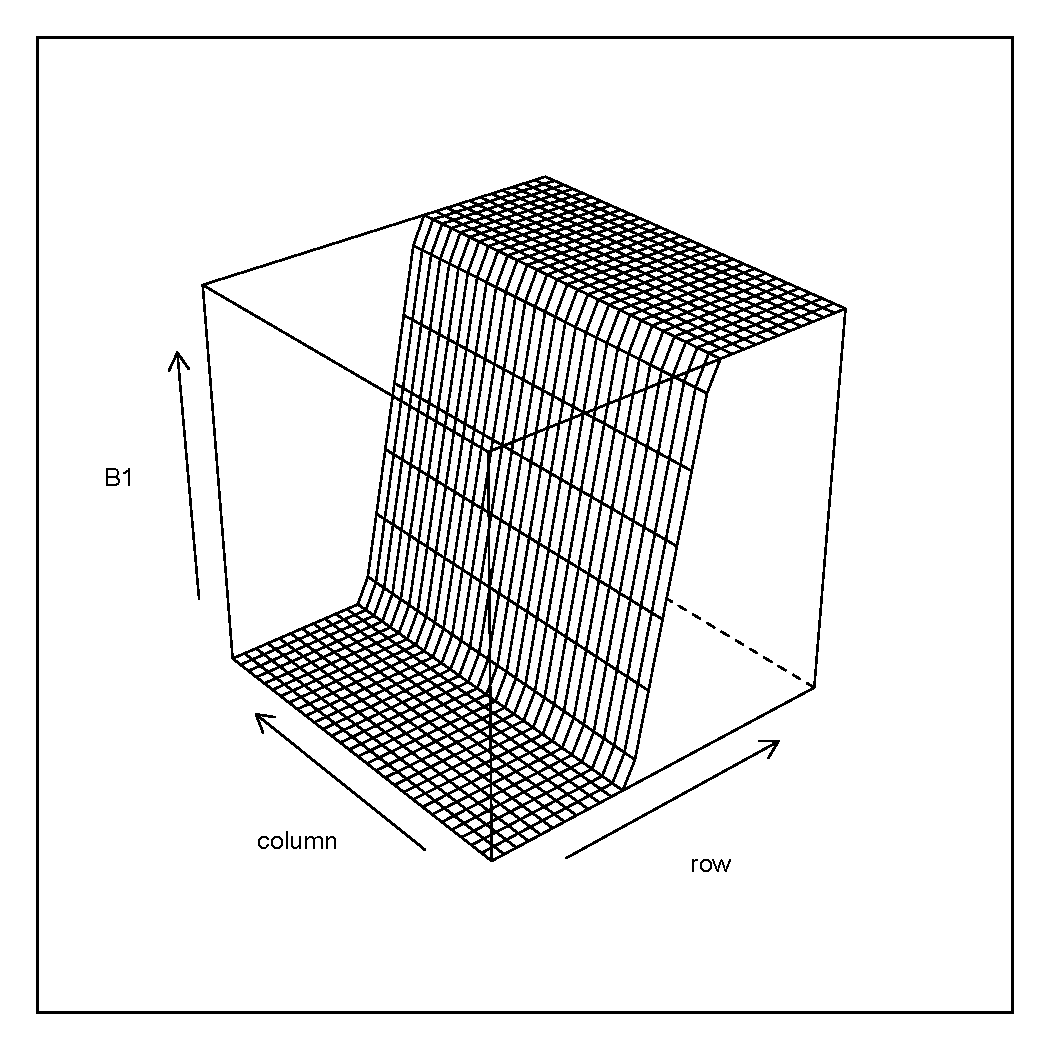
\includegraphics[width=0.32\textwidth]{../../figures/simulation/step.pdf}
			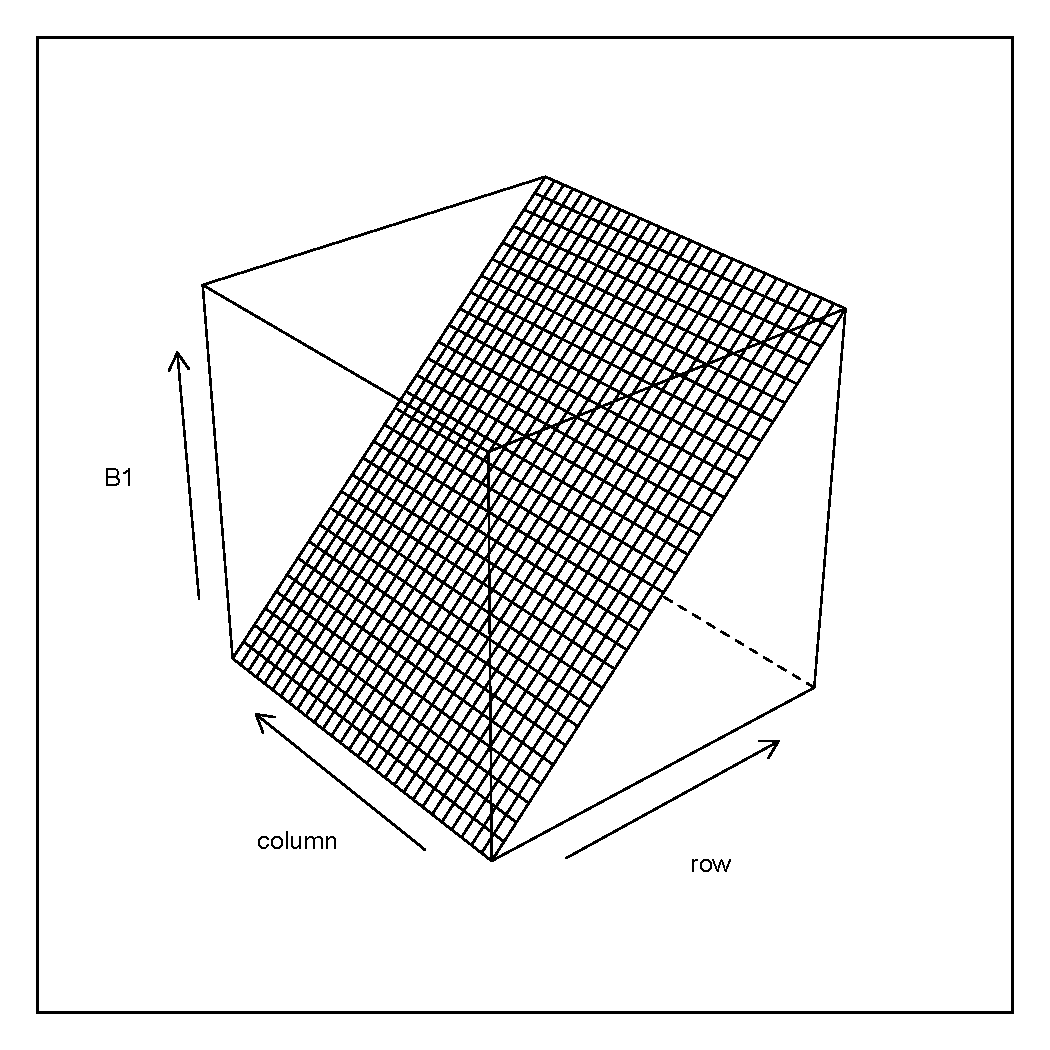
\includegraphics[width=0.32\textwidth]{../../figures/simulation/gradient.pdf}
			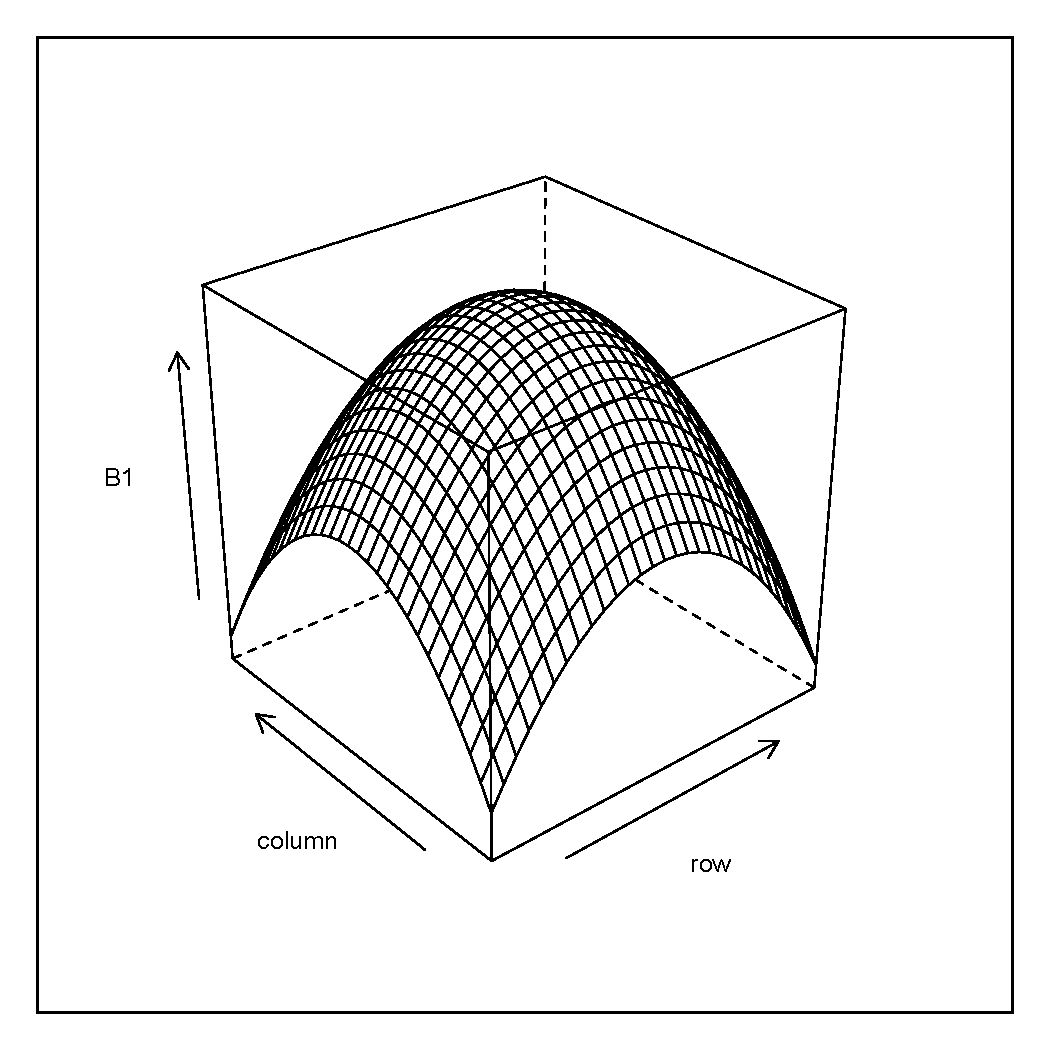
\includegraphics[width=0.32\textwidth]{../../figures/simulation/parabola.pdf}
			\caption{The actual $\beta_1$ coefficient surface used in the simulation.\label{fig:sim-actual}}
		\end{center}
	\end{figure}
	
	\begin{figure}
		\begin{center}
			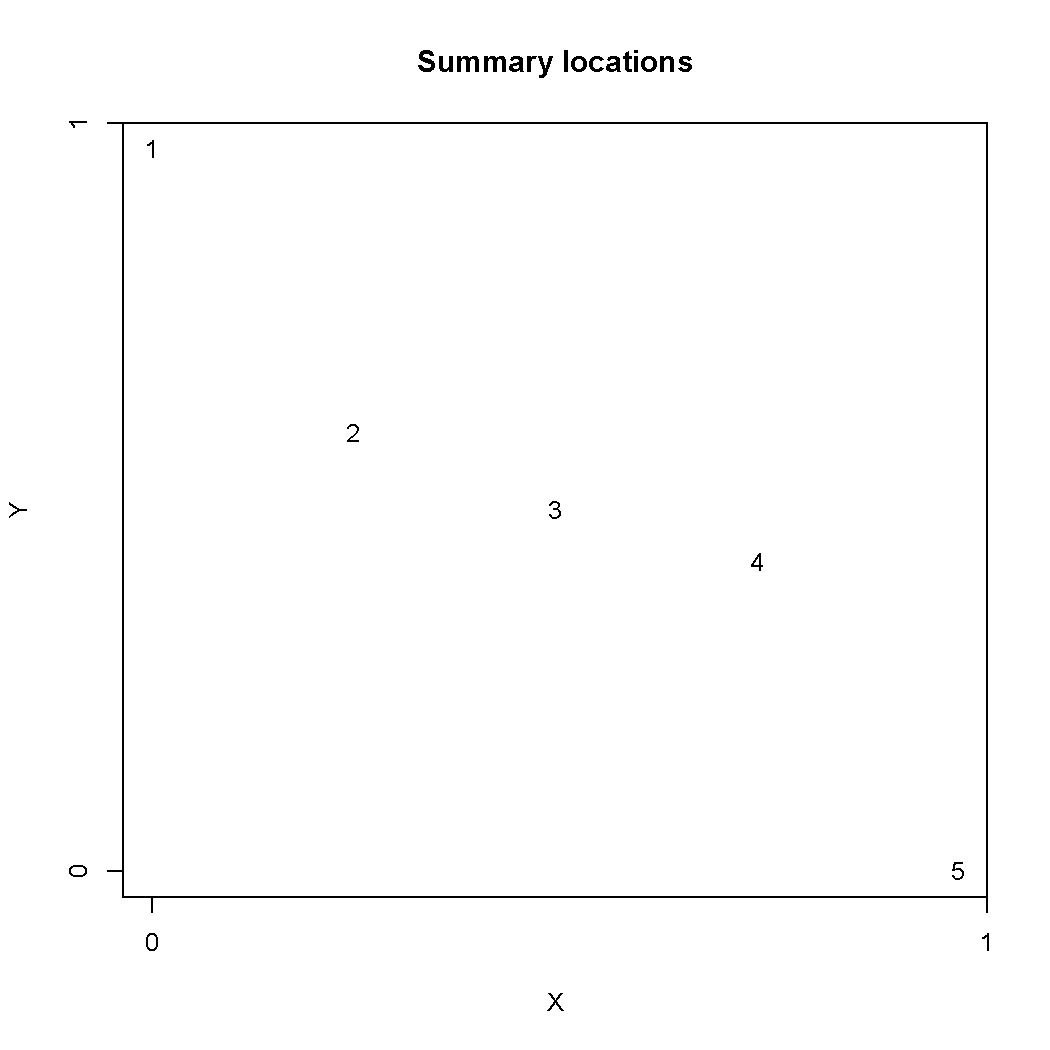
\includegraphics[width=0.5\textwidth]{../../figures/simulation/summary-locations.pdf}
			\caption{Locations where the variable selection and coefficient estimation of GWL were summarized.\label{fig:summary-locations}}
		\end{center}
	\end{figure}
	
	\paragraph{Summary locations}Results from the simulation were summarized at five locations on the domain (see Figure \ref{fig:summary-locations}). Locations one and five are at opposite corners of the domain, where we expect biased estimation from a kernel smoother like traditional GWR, particularly when the quantity being estimated has a nonzero gradient at the boundary, which is the case for the gradient and parabola functions. Because the GWAL and GWAEN use locally linear fitting, they are expected to exhibit less bias at the boundaries.
	
	Locations two and four are at the `corners' of the step function. Because the step function is undifferentiable at these locations, locally linear fitting is not expected to be as effective at reducing bias here as in the case of the boundaries of the gradient and parabola functions. Local variable selection is expected to be ambiguous at location four of the step function because it is at the the boundary where the coefficient transitions from zero to nonzero.
	
	All three coefficient functions are zero at location five. The parabola is also zero at location one. In these cases where the coefficient at the boundary but not elsewhere, the local variable selection is expected to be ambiguous because the data come almost entirely from locations where the coefficient is nonzero.
	
	Unlike the other two functions, the gradient is actually constant across the domain in terms of the covariate-by-location interaction. As a result, the optimal kernel bandwidth $\phi$ is expected to be larger for estimating the gradient coefficient surface than for the step or the parabola. The result should be that the estimation is more accurate for the gradient function in terms of bias, variance, and MSE.
	
	%Results of the simulation experiment were summarized to asses the consistency in selection and estimation, as well as the coverage properties of the confidence intervals. The confidence intervals based on the bootstrap (without shrinkage) were used for the GWL because they seemed to uniformly outperform the other options.\\ table:loc1-X1-BiasX
	
		
	\subsection{Simulation results}
	%At locations where $\beta_1$ is nonzero, $X_1$ usually selected for inclusion in all or nearly all of the model runs. An exception is at location four for the step function, where $X_1$ was included in about half of the model runs. This is probably because location four is at the very point where $\beta_1$ transitions from zero to nonzero. Selection performance was relatively poor for the step function at location one, especially for data with $\sigma^2 = 1$. For those simulations, $X_1$ was correctly included in around 85\% of the simulations. The bias, variance, and MSE of $\hat{\beta}_1$ under the same settings were also much larger than the baseline established by the standard \verb!gwr! algorithm. The reason(s) for the poor performance under those particular conditions is currently unknown.\\
	
	\paragraph{Selection} Table \ref{table:selection} lists the results of variable selection. The correct covariate was usually included in the local models, and the unimportant covariates were usually excluded. Arguably the least-accurate selection was at locations one and five for the step function using the {\tt lars} algorithm, where variables that do not appear in the true model were selected for inclusion at rates between 11\% and 22\%. The {\tt enet} and {\tt glmnet} algorithms, using the same data, had false-positive errors at rates between 0\% and 8\%, which are typical of the error rates for all other location/function/algorithm combinations.
	
	Selection performance was more affected by an increase in the noise variance from $\sigma_{\varepsilon}=0.5$ to $\sigma_{\varepsilon}=1$ than by an increase in colinearity from $\rho = 0$ to $\rho = 0.5$. For instance, for the step function at location three, $\beta_1(\bm{s}_3) = 0.5$. Where $\sigma_{\varepsilon}=0.5$, the {\tt glmnet} algorithm selected $\beta_1(\bm{s}_3) $ for inclusion at a rate of 100\% (when $\rho = 0$) and 99\% (when $\rho = 0.5$). But when $\sigma_{\varepsilon}=1$, the same algorithm selected $\beta_1(\bm{s}_3)$ for inclusion at a rate of 75\% (when $\rho = 0$) and 68\% (when $\rho = 0.5$).
	
	The \verb!enet! algorithm outperforms the others in selection but the difference is small - a roughly one percentage point improvement in the rate of true positives and true negatives when $\rho = 0.5$.There is no apparent difference between {\tt glmnet} and {\tt enet} when $\rho = 0$.  
	
	%Otherwise, selection performance was good, with the rate of false positive selections for $X_2$--$X_5$ (and for $X_1$ where its true coefficient was zero) usually below 0.10. Selection (also bias, variance, and MSE of $\hat{\beta}_1(\bm{s})$) tended to suffer worse by the change from low to high error variance than by the change from low to high collinearity amongst the predictors.\\
	
	\paragraph{Coefficient Estimation} The MSE, bias, and variance of $\hat{\beta}_1$ are listed in Tables \ref{table:X1-mse}, \ref{table:X1-bias}, and \ref{table:X1-var}, respectively. The method of oracular selection led to the best MSE in 28 of the 60 cases, which is more than any other single method. In general, the methods that do local variable selection had lower MSE than traditional GWR. As was the case for selection, estimation accuracy (in terms of MSE) suffered more by an increase in $\sigma_{\varepsilon}$ from 0.5 to 1 than from an increase in $\rho$ from 0 to 0.5. Oracular selection was decisively superior to traditional GWR and to local variable selection for estimating the gradient $\beta_1$, turning in the best MSE for all combinations of location and simulation parameters.
	
	In general, oracular selection and traditional GWR were quite similar in terms of $\text{var}\left(\hat{\beta_1}\right)$, with notably greater variance for the local selection methods. However, the local selection methods had less bias than traditional GWR, even exhibiting less bias than oracular selection in many settings. There was no simulation setting for which traditional GWR had the smallest or second-smallest bias.
	
	It seems, therefore, that the local selection methods reduce bias and increase variance of the coefficient estimates, as compared to traditional GWR. Whether traditional GWR or local selection is better in terms of MSE of the coefficient estimates is not clear in all cases, but when the actual coefficient is equal to zero (or nearly so), local selection does seem to reduce the MSE over traditional GWR.
	
	\paragraph{Autocorrelated Errors} Introducing autocorrelation in the errors causes a substantial degradation in the estimation accuracy of the GWAL and GWAEN, accompanied by a tendency to prefer smaller kernel bandwidths. The likely explanation is that when the kernel bandwidth is small, autocorrelated errors are indistinguishable from a varying intercept. The residuals are reduced to the extent that the errors are incorporated in the intercept term. Since this effect is absent in the case of uncorrelated errors, greater autocorrelation in the error term will tend to mean a greater reduction in the errors - and therefore a greater increase in the log likelihood - as the kernel bandwidth decreases.
	
	Since the optimal kernel bandwidth is balance between the log likelihood and the degrees of freedom consumed by the model, and because the effect of autocorrelated errors is an increase in log likelihood without an offsetting increase in the consumed degrees of freedom at a given kernel bandwidth, greater autocorrelation will tend to lead to a smaller optimal kernel bandwidth.
	
	This is an example of the bias-variance tradeoff: Accounting for the random noise within the systematic portion of the model decreases the bias but increases the variance.
	
	%There was not a clear and consistent difference in performance between the three selection methods. It might be expected that the adaptive elastic net would outperform the adaptive Lasso under greater covariate collinearity, but if such effect is real it is not apparent from this simulation. The unshrunk coefficient-estimation methods tended to exhibit more bias than the selection-plus-shrinkage methods when the true coefficient value was near zero, and vice versa when the true coefficient was not near zero. The unshrunk methods were perhaps more consistent in their performance and for that reason they are probably preferable in practice.\\
	
	%Bias in coefficient estimation was greater and variance less for the standard \verb!gwr! algorithm than for the methods described here. This is probably due to the fact that the methods described here show a preference for smaller bandwidths than those select by \verb!gwr!. Accuracy (as measured by MSE) in fitting the true Y variables was comparable for all the methods. \\	
	
	\paragraph{Fitted Values} The MSE of the $\hat{Y}$, $\text{MSE}\left(\hat{Y}\right)$, is listed in Table \ref{table:Y-mse}. Nominally, $\text{MSE}\left(\hat{Y}\right)$ should be equal to the noise variance, $\sigma_{\varepsilon}^2$, which is 1 for odd-numbered rows and 0.25 for even numbered rows. There is not much difference in $\text{MSE}\left(\hat{Y}\right)$ between the various estimation methods, except that it is larger for the oracular and \verb!gwr! methods where $\beta_1(\bm{s})$ is near or equal to zero.
	
	\subsection{Tables}
		\subsubsection{Selection}
			\input{../../output/simulation/selection}

		\subsubsection{Estimation}
			\input{../../output/simulation/msex}
			\input{../../output/simulation/bx}
			\input{../../output/simulation/varx}			
			\input{../../output/simulation/msey}

			
\section{Data Analysis\label{section:data-analysis}}
	\subsection{Census Poverty Data}
	An example data analysis is presented to demonstrate application of the GWAEN for local variable selection in an SVCR model of how poverty is related to a list of socio-economic variables. The data is from the U.S. Census Bureau's decennial census in the year 1960. This analysis looks specifically at the upper midwestern states of Minnesota, Iowa, Wisconsin, Illinois, Indiana, and Michigan. This is areal data, aggregated at the county level.
	
	Three kinds of variables  were considered as potential predictors of county-level poverty rate.
	\begin{itemize}
		\item Covariates that describe the county's employment structure ($\verb!pag!$, the proportion of residents employed in agriculture, $\verb!pex!$, the proportion of residents employed in mining, $\verb!man!$, the proportion of residents employed in manufacturing, $\verb!pfire!$, the proportion of residents employed in finance, insurance, and real estate, $\verb!pserve!$, the proportion of residents employed in services, and $\verb!potprof!$, the proportion of residents employed in other professions)\\
		\item Covariates that describe the county's racial makeup ($\verb!pwh!$, the proportion of residents who are white, $\verb!pblk!$, the proportion of residents who are black, and $\verb!phisp!$, the proportion of residents who are hispanic)\\
		\item $\verb!pmetro!$: an indicator of whether the county is in a metropolitan area.
	\end{itemize}
	The response variable (poverty rate) is a proportion, taking values in $[0,1]$. To demonstrate the geographically-weighted Lasso in a linear regression context, we model the logit-transformed poverty rate. The predictor variables were not transformed - raw proportions were used.
	
	\subsection{Modeling}	
	The adaptive elastic net was used for variable selection, and then coefficients for the selected variables were estimated by weighted least squares without shrinkage. The standard {\tt gwr} algorithm was used to fit a model to the same data for the sake of comparison.
	
	\subsection{Figures}
	The coefficient estimates are plotted on maps of the upper midwest in Figure \ref{fig:unshrunk-enet-coefs-1960} (based on the AEN) and Figure \ref{fig:gwr-coefs-1960} (for traditional GWR).
	\begin{figure}
		\begin{center}
			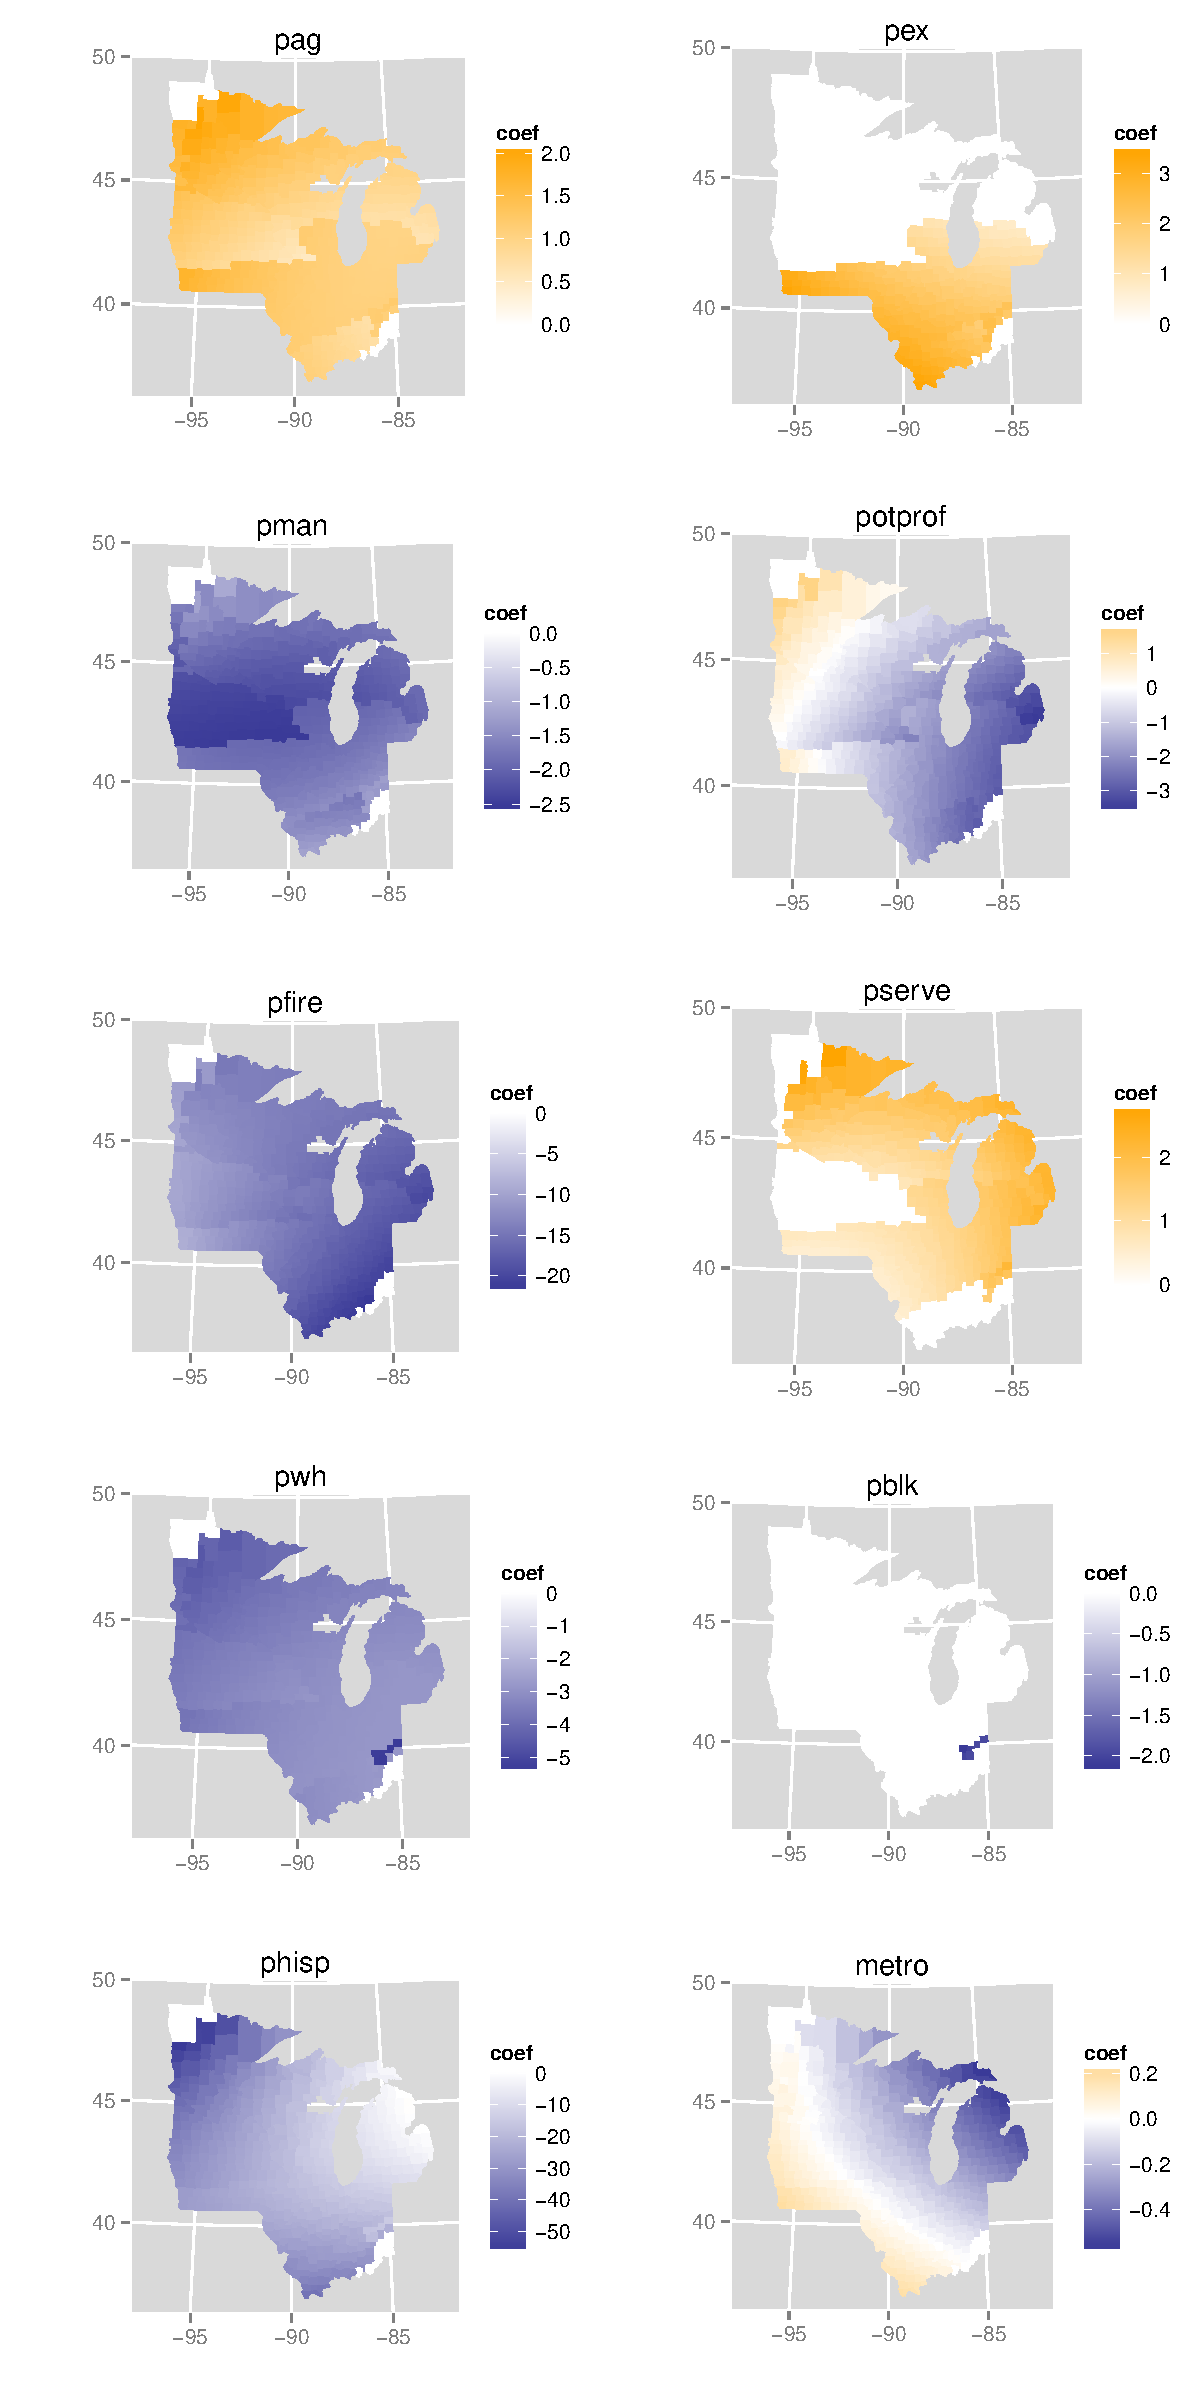
\includegraphics[height=8in]{../../figures/poverty/1960-enet-linear-coefficients-unshrunk.pdf}
			\caption{Coefficient surfaces for the logit of poverty rate, based on the 1960 census and selected by the AEN. \label{fig:unshrunk-enet-coefs-1960}}
		\end{center}
	\end{figure}	
	
	\begin{comment}
	\begin{figure}
		\begin{center}
			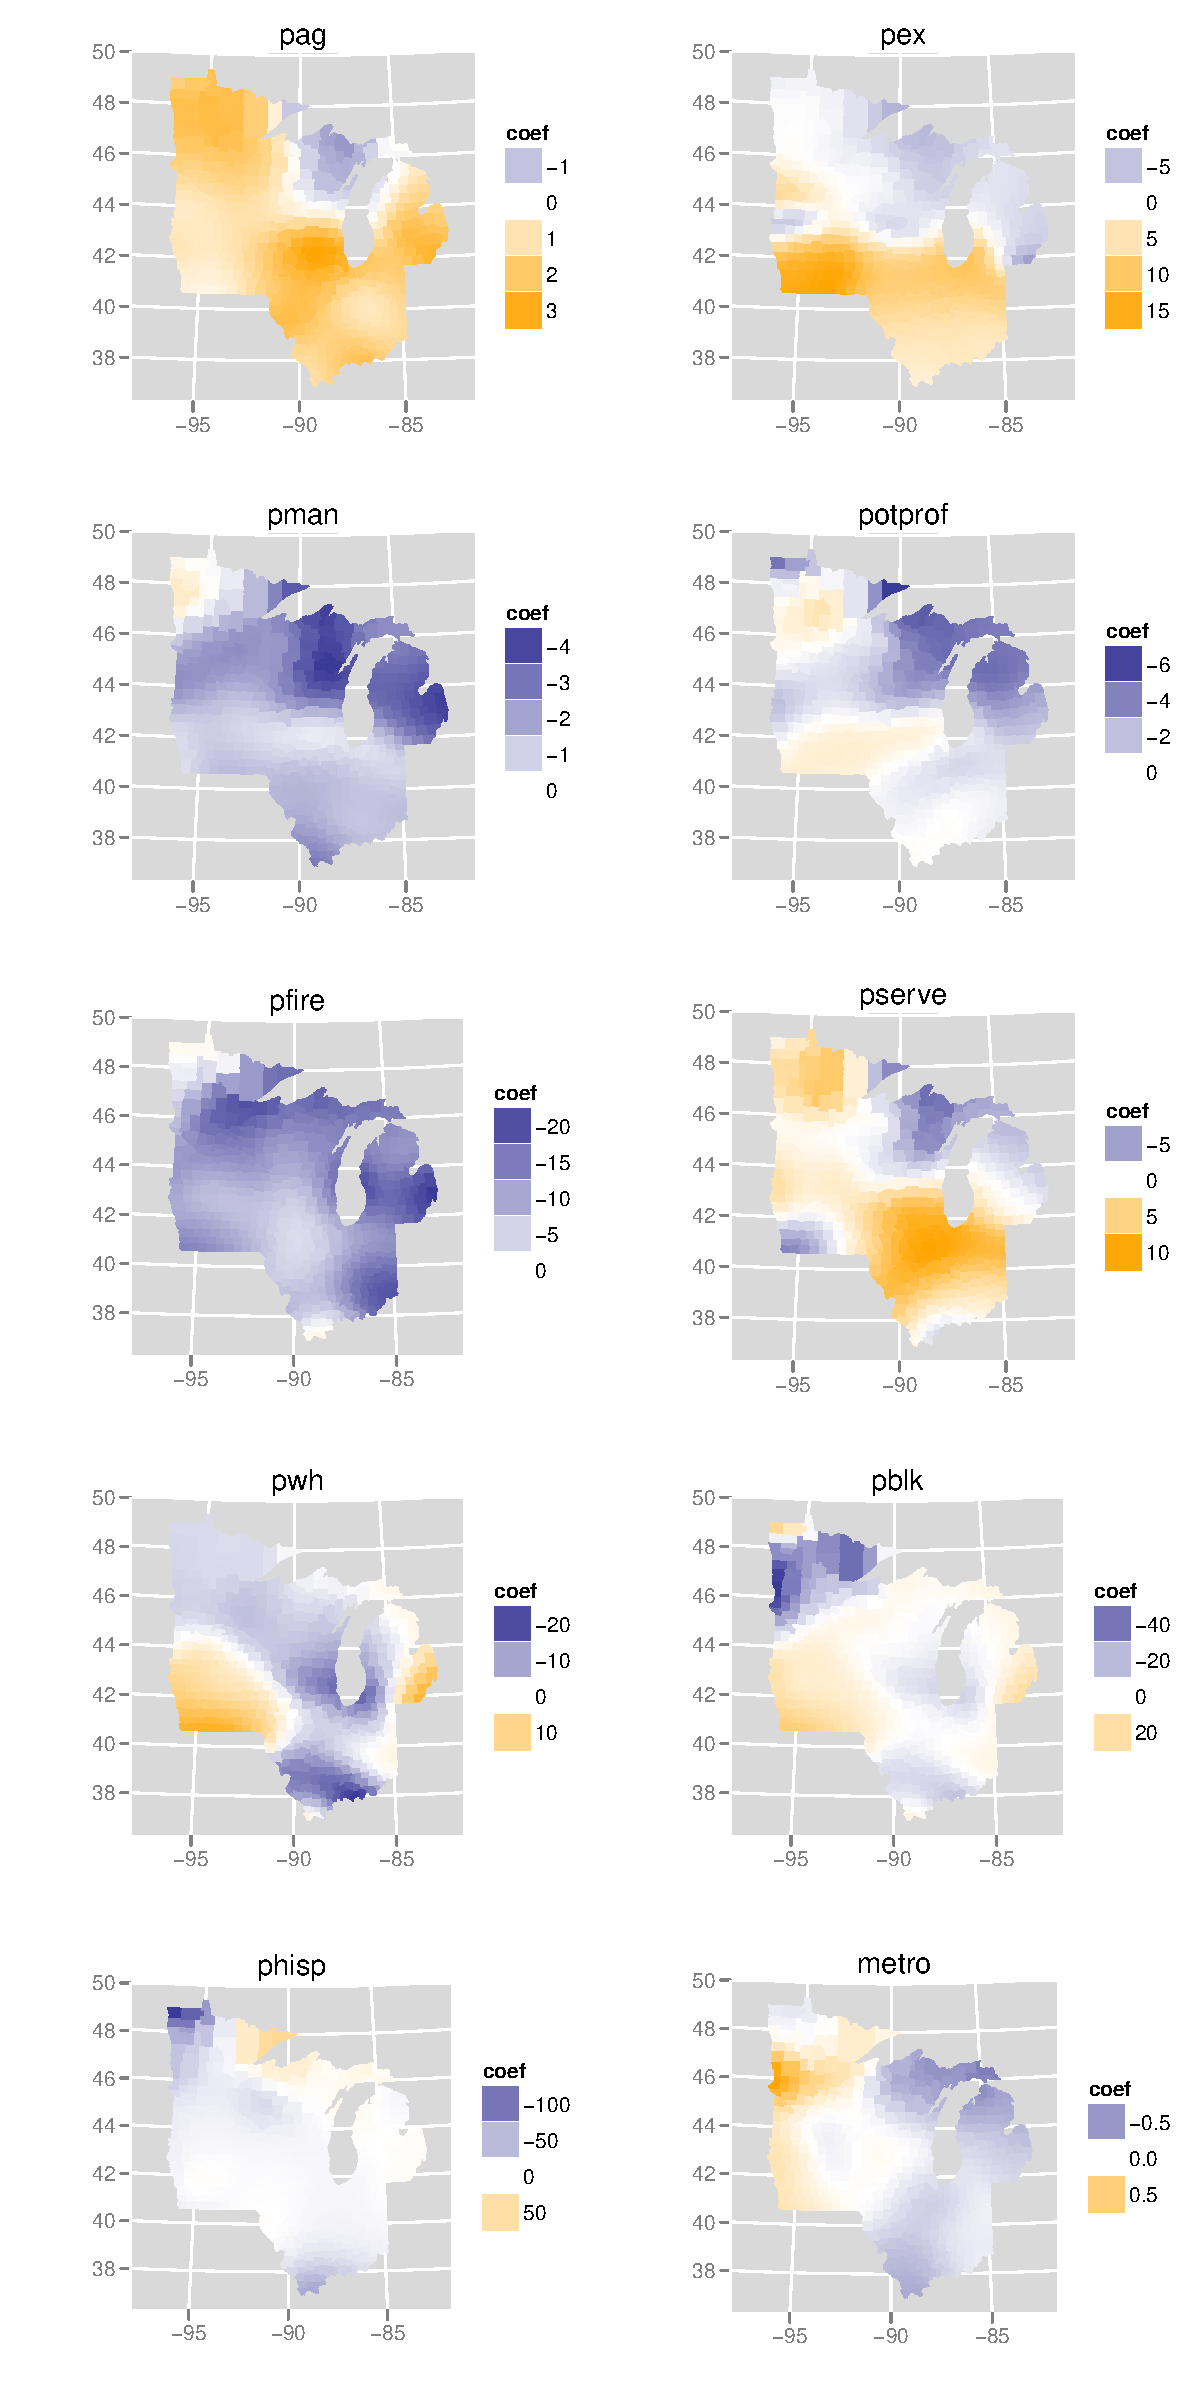
\includegraphics[height=8in]{../../figures/poverty/1970-gwr.pdf}
			\caption{Coefficient surfaces for the logit of poverty rate based on the 1970 census and estimated by traditional GWR. \label{fig:gwr-coefs-1970}}
		\end{center}
	\end{figure}
	\end{comment}	
			
	\subsection{Discussion}
	It is immediately apparent that the estimated coefficient surfaces are non-constant for most variables. The same large-scale patterns appear in both figures, but with differences. First of all, the AEN has selected a larger bandwidth than traditional GWR, so there is less variability in the coefficient estimates from the AEN. This may be one reason that the AEN coefficient estimates are less extreme than those for traditional GWR. In a model with a logit-transformed proportion as the output, the coefficients can be interpreted as log odds ratios, so, e.g., the estimate of -100 as the coefficient of \verb!phisp! (albeit at the edge of the domain) seems unrealistic.
	
	Assessing variable selection for this data is difficult, since the AEN almost never removed any variables from the model. Indeed, some coefficients seem nearly constant across the domain. An exception is the coefficient surface for \verb!pex! (mining employment). That surface indicates an interaction whereby the proportion of people working in mining in southern parts of the domain is associated with an increase in the poverty rate, while in northern parts of the domain it is associated with a decrease in the poverty rate.

%\end{spacing}

\section{References}
\bibliographystyle{chicago}
\bibliography{../../references/gwr}

\end{document}  